\section{Motivations}
\subsection{Fallacy: LBA-based lifetime prediction}

Current automatic methods predict the lifetime of data based on the update
frequency of LBAs~\cite{AutoStream}.  
For example, AutoStream~\cite{AutoStream} assumes that, if
some LBAs are frequently rewritten by applications, those LBAs hold hot data.
This LBA-based lifetime prediction works poorly on modern applications, where
the majority of new data are written in an append-only manner.  To understand
the correlation between LBAs and the lifetime of data under append-only
workloads, we analyzed the write pattern of RocksDB~\cite{RocksDB}, which is a
popular key-value store based on the LSM-tree algorithm~\cite{LSM}.

Figure~\ref{fig:lba_lifetime}(a) shows the lifetime distribution of data
according to LBAs. Here, the lifetime of data is defined to be 
a number of write requests between when the data is written 
to when the data is invalidated an overwrite or a TRIM command. 
%an elapsed time (unit: $\mu$sec) from when it is newly written to a certain LBA to when it is
%invalidated by an overwrite or a TRIM command. 
As shown in
Figure~\ref{fig:lba_lifetime}(a), there is no strong correlation between the
lifetime and LBAs -- all the data have very different lifetimes, regardless of
their LBA numbers. We also observed how the lifetimes of LBAs changed according
to the time in a more microscopic view.  For a small number of consecutive LBAs
(256 LBAs), composing a 1 MB chunk, 
we plot the trend of the lifetime of the chunk for 630 data
in Figure~\ref{fig:lba_lifetime}(b). As shown in the figure, the LBAs belonging
to the chunk first hold hot data. For example, at the logical time
10, the lifetime of the chunk is close to 1 requests.  
At the logical time 450, however, its lifetime increases to
2.6 million requests. Then, the lifetime drops to 1.2 million
requests at 600 logical time.  Consequently, our observations shown in
Figure~\ref{fig:lba_lifetime} indicate that, under append-only
workloads, LBAs couldn't be a useful metric that decides the hotness or
lifetime of data that they hold.

\begin{figure}[t]
	\centering
	\subfloat[Lifetime patterns over LBAs]{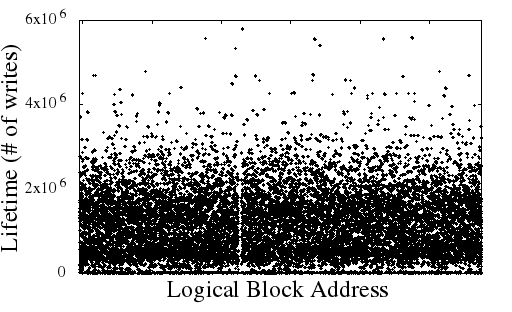
\includegraphics[width=0.25\textwidth]{figure/lba_lifetime2}}  % data from 0/03031641
	\subfloat[Lifetime patterns over time (for a fixed LBA range)]{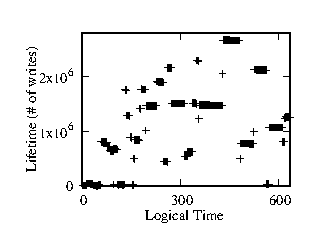
\includegraphics[width=0.22\textwidth]{figure/lifetime_in_chunk2}}
	%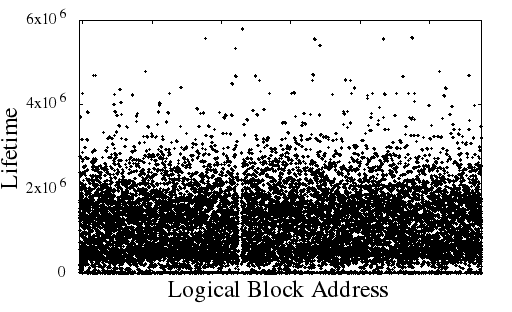
\includegraphics[width=0.9\linewidth]{figure/lba_lifetime} 
	\vspace{-10pt}
	\caption{
		Data lifetime distributions over varying LBAs and logical times.
		\textcolor{red}{(TODO:) it would be good to include same graphs with
		in-place update workloads;}}
		\label{fig:lba_lifetime}
	\vspace{-15pt}
\end{figure}

\subsection{Program context as a lifetime predictor}

In order to properly assign data to a specific stream in accordance with their
lifetimes, it is necessary to find a new metric for lifetime prediction.  It is
obvious that append-only applications write data with different lifetimes.  For
example, RocksDB appends write-ahead logs to storage to ensure data
persistence.  Those logs have short lifetimes because they are quickly deleted
(or trimmed) after original data are safely stored in the persistent storage.
The flush module of RocksDB (which materializes the content of a memtable in
DRAM, often called a L0 table, to a L1 table in the storage) generates data
with relatively short lifetimes. This is because a L1 table will be flushed to
a L2 table and be removed in the near future. Conversely, a compaction module
often writes long-lived data that are unlikely to be removed for a long time.

The above observation implies that, if we are able to know the detailed
behaviors of append-only applications, data with different lifetimes can be
isolated in separate streams in an SSD. As mentioned in Section~\ref{sec:intro}, a
common solution~\cite{MultiStream} to realizing this is manually modify an
application code so that each module assigns a unique stream ID to data stream
it generates. However, owing to considerable implementation efforts
required to modify individual applications, this approach is not widely used in
real-world environments.

In this paper, we claim that a program context is a useful tool that delivers
the information of data lifetimes to the storage side without modifying application
code manually. The program context is calculated at runtime by summing the
values of program counters that are identified along function-call paths
of an application.  Logging, flushing, and compaction are invoked through
different function-call paths.  Thus, by leveraging the program context, we are
able to identify software modules that generate specific write streams.  Note
that using the program context to identify characteristics of data is not new.
Ha \textit{et al.} proposed a way of separating hot-cold data by referring to the program
context~\cite{PCHa}. This work, however, was not designed for append-only
applications and didn't take into account the use of a multi-stream feature of
a modern SSD.

\begin{figure}[!t]
\centering
\hspace{1pt}
\subfloat[manual: log]{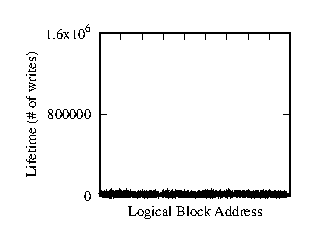
\includegraphics[width=0.23\textwidth]{figure/type_1b}} % data from 4/03031953 
\subfloat[PC\#2]{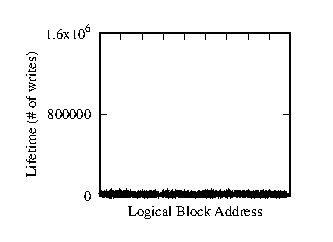
\includegraphics[width=0.23\textwidth]{figure/pcID_2b}}
\hfill
\vspace{-10pt}
\subfloat[manual: flush] {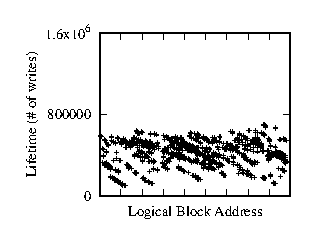
\includegraphics[width=0.23\textwidth]{figure/type_3b}}
\subfloat[PC\#3]{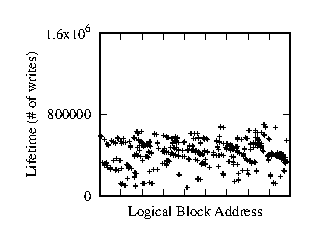
\includegraphics[width=0.23\textwidth]{figure/pcID_3b}}
\caption{Data lifetime distributions of different PCs.} 
\label{fig:types_and_PCs}
\vspace{-20pt}
\end{figure}

In order to confirm our hypothesis that the program context could provide
enough information to recognize detailed behaviors of an application, we
conducted a series of experiments using RocksDB, comparing the accuracy of
lifetime prediction by two different methods: 1) when the type of data streams
is manually identified by modifying the code (\texttt{manual}) and 2) when the
stream type is automatically tagged by the program context
(\texttt{automatic}).  Figure~\ref{fig:types_and_PCs} compares the lifetime
distributions of data that are separated by \texttt{manual} and
\texttt{automatic}.  Figures~\ref{fig:types_and_PCs}(a) and (b) represent how
well the two methods identify log data written by
RocksDB.  As mentioned earlier, log data are short-lived, and the
\texttt{automatic} method with the program context shows high accuracy
comparable to \texttt{manual}. Similarly, Figures~\ref{fig:types_and_PCs}(c)
and (d) shows the accuracy of identifying data streams written by the flush
module of RocksDB.  As expected, these two graphs have the similar lifetime
patterns, which proves that the program context can be a good lifetime hint.


%because the data in memory
%is temporarily maintained until the data is flushed to the storage for the
%consistency reason~\cite{RocksDB}.


%In order to verify that the PC information is enough to recognize the behavior
%of these applications, we ran RocksDB and compared the data lifetimes when the
%type of data was manually identified aginst when the data is identified by PC
%values.  Figure~\ref{fig:types_and_PCs} shows the lifetime distribution of data
%separated by manual scheme and PC values for two cases, i.e., log and flush.
%First, Figure~\ref{fig:types_and_PCs}(a) represents the lifetime of the log
%file of RocksDB.  RocksDB's log data is short-lived because the data in memory
%is temporarily maintained until the data is flushed to the storage for the
%consistency reason~\cite{RocksDB}.  Figure~\ref{fig:types_and_PCs}(b) depicts
%the data lifetime of ID 2 among the classified PCs according to the our
%proposed collection method.  As these two graphs have the same lifetime
%pattern, we can say PC ID 2 represents the context of the log file.  Similary,
%Figure~\ref{fig:types_and_PCs}(c) shows the lifetime of flushed static sorted
%table (SST) files of RocksDB.  The flush operation stores the memory data as an
%SST file at level 0 of the LSM tree in the storage.  The file is deleted by a
%compaction operation that removes invalid data when each level is full.  Due to
%the characteristics of the LSM tree, which becomes smaller as it goes to top
%level, the compaction is often performed at level 0, so the flushed data at
%level 0 has a relatively short lifetime~\cite{RocksDB}.
%Figure~\ref{fig:types_and_PCs}(d) shows data lifetime of PC ID 3.  As expected,
%these two graphs have the similar lifetime patterns proving the PC can be a
%good lifetime hint.


% commentated
\begin{comment}
Recently, various studies are proposed to exploit the stream feature in two .
First, Kang et al.~\cite{MultiStream} proposed that the application
is modified to manually assign streams.
Since an application knows the lifetime of the data best, this approach
is very effective in reducing WAF.
However, in order to properly specify streams in the application, the programmer must
fully understand the lifetime characteristics of the data.
Also when multiple applications try to assign streams, a centralized stream assignment
is required to avoid conflicts.
Second, FStream~\cite{FStream} separates short-lived data, e.g., file system metadata and
journal, using the file system information. 
FStream does not require a burden on the programmer, but the system developer is still burdened
to identify short-lived data of the application, e.g., log data of key-value store, based on the file extension.
In addition, those manual techniques are unable to adapt the stream mapping when the workload or application changes.
These limitations of the manual approach can be overcome by the automatic approach.
Lastly, unlike other schemes, AutoStream~\cite{AutoStream} is aimed to automate the process of mapping 
write I/O operations to an SSD stream.
However, since AutoStream relies on the past LBA access patterns, it is not practical when the data are written in
append-only manner, as modern key-value store.
\end{comment}


